\documentclass{article}
\usepackage[brazilian]{babel}
\usepackage[utf8]{inputenc}
\usepackage{amsmath,amsfonts,amstext}
\usepackage{hyperref}


\usepackage{booktabs}
\usepackage{geometry}
\usepackage{graphicx}
\usepackage{subfig}

\title{Implementação digital de um Minimoog}
\author{Bruno Figueira Lourenço \\ Jonathan Alis Salgado Lima}

\begin{document}
\maketitle

\section{Introdução}


O objetivo desse trabalho foi fazer uma implementação digital de um Minimoog em forma de \emph{plugin} VSTi.



\section{Arquitetura Geral do Sistema}



A implementação do Minimoog foi divida em duas partes, que correspondem às 
duas pastas na estrutura de diretórios do projeto:

\begin{itemize}
	\item \emph{src} - Contém as classes responsáveis por efetuar 
	a síntese de áudio propriamente dita. Foram implementadas diversas 
	unidades básicas. A classe \emph{Moog} conecta essas unidades básicas para 
	emular a estrutura do Minimoog. Esta pasta também contém um diretório 
	de testes (\emph{Tests}) para os blocos de síntese construídos.
	\item \emph{plugin} - Contém as classes responsáveis por fazer a 
	interface entre a síntese de áudio e a API VST.
\end{itemize}

\section{Síntese de Áudio}


\begin{figure}
\centering
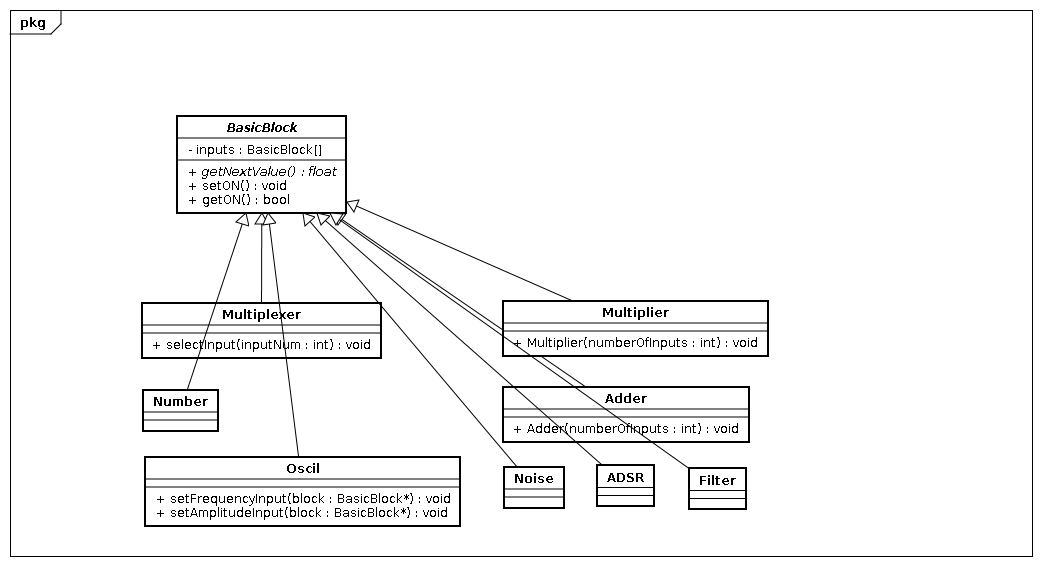
\includegraphics[scale=0.4]{Classes.png}\caption{Diagrama UML dos blocos básicos de síntese}\label{fig:uml1}
\end{figure}


Para implementar o Moog, optou-se por dividir em diversos blocos básicos, 
que representam cada um dos blocos que compõem o instrumento. Para isso, 
criou-se a classe \emph{BasicBlock} (\emph{basic\_blocks.h}) que representa 
uma unidade básica de síntese. A Figura \ref{fig:uml1} mostra o diagrama 
de classes correspondente.


Para construir a arquitetura de um minimoog, precisaremos de diversos blocos básicos para passar os dados da forma como queremos,
 e poder organizar a arquitetura.
Todos os blocos de síntese herdam da classe \emph{BasicBlock} e sobrescrevem 
o método \emph{getNextValue}, que é o responsável por obter a próxima 
amostra de áudio do bloco. A classe \emph{BasicBlock} também fornece métodos 
para ligar(\emph{getON} e \emph{setON}) e resetar (\emph{resetBlock}) a unidade.

Naturalmente, a semântica de ``ligar'' e ``resetar'' o bloco varia de unidade para unidade. 
Por exemplo, se desligarmos um \emph{Oscil} e chamarmos \emph{getNextValue}, a unidade 
retornará $0$. Já no caso da classe \emph{Filter}, desligar o filtro significa que não 
será feito processamento e o sinal será devolvido tal como recebido pelo filtro. 

Finalmente, através do método \emph{setInput} é possível usar um outro \emph{BasicBlock} 
como entrada para a unidade em questão. Por exemplo, a classe \emph{Oscil} recebe 
dois \emph{BasicBlock} como entrada, um representando a frequência e o outro 
a amplitude de oscilação.

Todos os blocos estão definidos no arquivo \emph{basic\_blocks.h} e implementados nos arquivos \emph{nomedaclasse.cpp}.

Nas subseções seguintes descreveremos alguns aspectos das classes derivadas de \emph{BasicBlock}.

\subsection{\emph{Number}}
A classe \emph{Number} serve para obtermos um número como sinal amostrado, usamos para obtermos um sinal de valor fixo. 
Ela não recebe nenhum outro bloco básico, é construida apenas com o valor do número. Essa classe tem um atributo com o valor do número 
e o método \emph{getNextValue} retorna esse número.
\subsection{\emph{Adder}}
A classe \emph{Adder} serve para podermos somar um número qualquer de sinais amostrados. Ao ser construída, deve-se passar o número de entradas,
 e ao usar deve-se indicar quais blocos básicos serão as entradas. Para obter a próxima amostra, o método \emph{getNextValue} obtém as próximas amostras de 
todos os blocos de entrada, via \emph{getNextValue} dos blocos básicos de entrada, e esses valores são somados e esse valor é retornado.
\subsection{\emph{Multiplier}}
A classe \emph{Multiplier} serve para podermos multiplicar um número qualquer de sinais amostrados. Funciona de forma análoga ao \emph{Adder}, mas a operação e de multiplicar.
\subsection{\emph{Multiplexer}}
O multiplexador, implementado na classe \emph{Multiplexer} funciona como um seletor de uma das entradas. Ele também recebe um número arbitrário de blocos 
básicos ao ser construído, e também devem ser escolhidos quais são esses blocos. O método setSelectedInput escolhe qual bloco passará para a saída, 
a partir de um parametro inteiro. O retorno do método \emph{getNextValue} será a próxima amostra do bloco escolhido obtida pelo método \emph{getNextValue} do bloco escolhido.
\subsection{\emph{Oscil}}
O bloco oscilador implementado pela classe \emph{Oscil}, é um dos blocos mais importantes para esse sintetizador, ele que gera o sinal rico em harmonicos que
 será processado, manipulado e filtrado para obter o som sintetizado como queremos.
Ele usa 2 blocos básicos que o controlam, a entrada de frequência e a entrada de amplitude, que são sinais que controlarão frequência e amplitude do oscilador, que são
selecionados a partir dos métodos \emph{setFrequencyInput} e \emph{setAmplitudeInput}. 


O método \emph{setWavetable} controla qual tipo de onda que o oscilador usará. Esses tipos de onda estão estruturados em uma classe chamada \emph{Waveform}, implementada no
arquivo \emph{Waveform.cpp} com os tipos de onda implementados, que são: triangular, dente de serra, quadrada, reta larga e reta estreita, que são colocados numa 
tabela usada pelo oscilador. O método \emph{getNextValue} da classe \emph{Oscil} faz o table lookup da Wavetable escolhida, de acordo com a frequência de entrada e
e usando interpolação linear para indices não inteiros, além de multiplicar pelo o valor de amplitude passado como entrada.


A classe \emph{Oscil} ainda faz sincronismos entre 2 osciladores. Se o atributo \emph{syncON} estiver com o valor TRUE, o que é feito pelo método
\emph{setSyncON}, e se um outro \emph{Oscil} foi escolhido como um oscilador escravo pelo método \emph{setSlave}, entao esse oscilador escravo é resetado 
no instante que o oscilador principal completa seu ciclo. Isso gera efeitos  bem interessantes que só sincronismo entre os osciladores proporcionam.

\subsection{\emph{Noise}}
O gerador de ruído implementado pela classe \emph{Noise} gera 2 tipos de ruídos, o ruído branco e o ruído rosa além de ter um bloco de entrada que controla a amplitude.


O ruído branco é o ruído gerado por números aleatórios(nesse caso, as limitações da computação faz com que sejam números pseudo-aleatórios),
 que contém todas as bandas de frequência com a mesma intensidade.



O ruído rosa é o ruído que tem todas as bandas de frequência, mas com intensidades proporcionais ao inverso da frequência, ou seja, para maiores
 frequências menos vai ser a intensidade dela. A implementação usada foi usando uma filtragem do ruído branco e está disponível em \url{http://www.firstpr.com.au/dsp/pink-noise/}.


O tipo de ruído pode ser selecionado através do método \emph{setType}, o bloco que controla a amplitude é selecionado pelo método \emph{setAmplitudeInput}
e o método \emph{getNextValue} retorna a uma amostra do ruído selecionado, multiplicado pelo bloco que controla a amplitude.

\subsection{\emph{ADSR}}
O ADSR é um controlador de envoltórias de amplitude e frequência, essa sigla representa o atack, decay, sustain e release, que são 
respectivamente o tempo de ataque, decaimento, o nível de sustentação e tempo de relaxamento de uma envoltória, onde ainda podemos 
escolher a declividade do atack, decay e do release além do valor do sustain.



Na classe \emph{ADSR} temos métodos para selecionar todos esses valores, temos os métodos \emph{attack\_function}, \emph{decay\_function}
 e \emph{release\_function}, que fazem o cálculo da curva de attack, decay e release simulando o circuito elétrico analógico. Ou seja, a curva da figura \ref{fig:ADSR}.



O método \emph{getNextValue} faz o cálcula qual o estágio corrente de acordo com os valores de attack, decay, sustain e release, e dependendo de 
qual estágio está, se chama o método correspondente, a menos no sustain, onde retorna o nível de sustain.


\begin{figure}
\centering
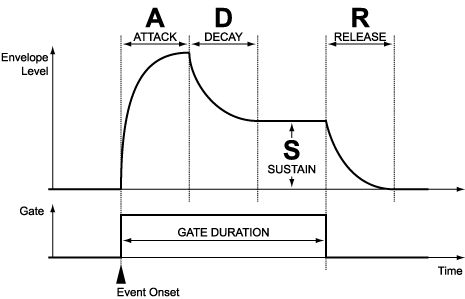
\includegraphics[scale=0.3]{ADSR.png}\caption{Curva de attack, decay, sustain e release.}\label{fig:ADSR}
\end{figure}

\subsection{\emph{Filter}}


O filtro é uma implementacao digital dos filtros controlados por tensao \emph{VCF} usados nos minimoogs, feito por Robert Moog baseado no 
trabalho descrito em \cite{moog_filter}. 
\subsubsection{Fundamentação teorica}
Esse filtro
 é uma construção em série de 4 filtros passa baixa implementados com circuitos RC, com resistencia variavel por tensao, podendo assim controlar a
 frequência de corte, além de uma realimentacao invertida multiplicada por um fator de qualidade ($k$) que varia de 0 a 4.
O comportamento dele é dependente do $k$, para $k=0$ ele atua como um passa baixa, com o crescimento de $k$, aparece uma elevacao 
cada vez mais acentuada na função de transferencia no valor da frequência de corte, e quando $k$ chega a 4 o filtro passa a oscilar.
Cada um dos 4 estagios do filtro pode ser representado pela função de transferencia

\begin{equation}\label{eq:(1)}
G(s) = \frac{\omega_c}{\omega_c+s}  
\end{equation}

Onde $\omega_c$ é a frequência de corte em radianos, e $s$ é a variável da Transformada de Laplace.
Ao serializar 4 esses filtros e introduzir uma realimentacao com o fator $-k$, a função de transferência fica

\begin{equation}\label{eq:(2)}
 H(s) = \frac{G(s)^4}{1+k G(s)^4} 
\end{equation}

\subsubsection{Discretização do filtro}

Para discretizar o filtro, usamos uma transformação bilinear para obtermos uma G(z) a partir da G(s), 
com uma nova estimativa do valor $\omega_c$, chamaremos essa estimativa de $\omega_c$~.
substituindo s por $(\frac{2}{T})(\frac{z-1}{z+1})$ em \ref{eq:(1)}, obtemos:

\begin{equation}\label{eq:(3)}
G(z) = b_0 \frac{1+z^{-1}}{1+a_1 z^{-1}}  
\end{equation}


Onde $b_0 = \frac{T \tilde{\omega_c}}{T \tilde{\omega_c}+2}$ e $a_1 = \frac{T \tilde{\omega_c} -2}{T\tilde{\omega_c} +2}$, onde $T$ é o período de amostragem.
Pela definicao de transformacao bilinear, a pulsacao antitransformada $\tilde{\omega_c}$ do filtro digital é

\begin{equation}\label{eq:(4)}
\tilde{\omega_c} = b_0 \frac{2}{T} \tan({\frac{T \omega_c}{2}} ) 
\end{equation}

Com isso temos a função de transferência de um estágio do filtro.

\subsubsection{Implementação digital do circuito}

Temos apenas a função de transferência, mas precisamos saber como obter o circuito que simula essa função de transferência.
Uma forma de obter o circuito é fazendo $G(z) = \frac{Y(z)}{X(z)}$, e igualando a \ref{eq:(3)} e isolando $Y(z)$, com isso obtemos


\begin{equation}\label{eq:(5)}
Y(z) = b_0(X(z)+X(z)z^{-1})-a_1Y(z)z^{-1}
\end{equation}

Usando a transformada inversa $z$:

\begin{equation}\label{eq:(6)}
y(n)=b_0(x(n)+x(n-1))-a_1 y(n-1)  
\end{equation}


Esse é o nosso $G(z)$, serializando 4 desses e acrescentando a realimentação, encontramos o circuito de que se obtém o filtro.


\subsubsection{A classe Filter}
Um objeto da classe Filter é criado com 
3 blocos básicos como entrada, sendo que o primeiro e o sinal que vai ser filtrado, a frequência de corte do filtro e o fator de qualidade, através dos
métodos \emph{setInputSignal}, \emph{setFrequencyInput} e \emph{setQualityInput}.
Como o próximo valor da saida do filtro depende das entradas e saídas anteriores de cada um dos estágios, foi nescessário criar os atributos
 para guardar os valores anteriores de entrada e saída de cada estágio. Eles são \emph{x\_1}[4] e \emph{y\_1}[4]. 


O método \emph{getNextValue} obtém $b0$ e $a1$ a partir dos valores dos blocos de entrada, faz a realimentação de acordo com o fator de qualidade, 
 faz o cálculo do valor de saída de cada estágio, segundo a equação \ref{eq:(6)}, atualiza os atributos \emph{x\_1}[4] e \emph{y\_1}[4] para terem o valor correto
 na próxima chamada do método \emph{getNextValue} e retorna o valor de saída do último estágio.

\subsubsection{Resultados}


Usando a classe \emph{Filter} conseguimos os seguintes resultados de uma análise de frequência em amostras de 2 segundos usando ruído branco como entrada do filtro
 a uma frequência  de corte $880 hz$. Os gráficos foram feitos com a ferramenta \emph{Espectro de frequência} do programa \emph{Audacity}.

\begin{figure}
  \centering
\parbox{1.5in}{
    \centering
    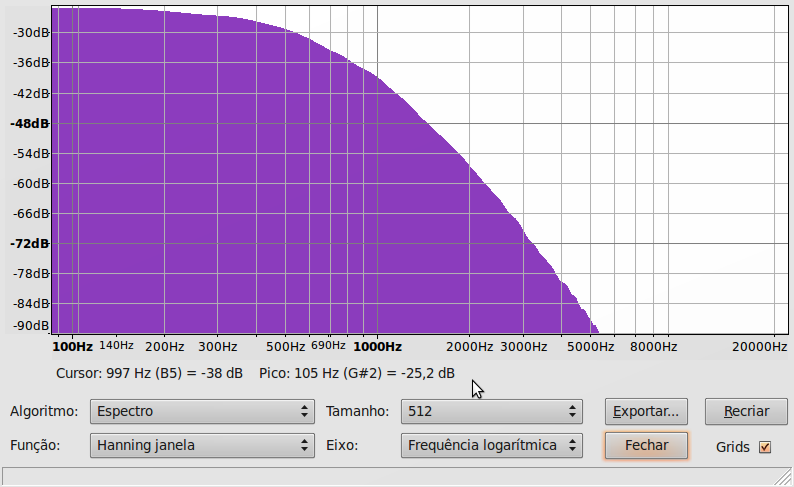
\includegraphics[scale=0.15]{q0.png}
    }%
\qquad	  
\parbox{1.5in}{
      \centering
      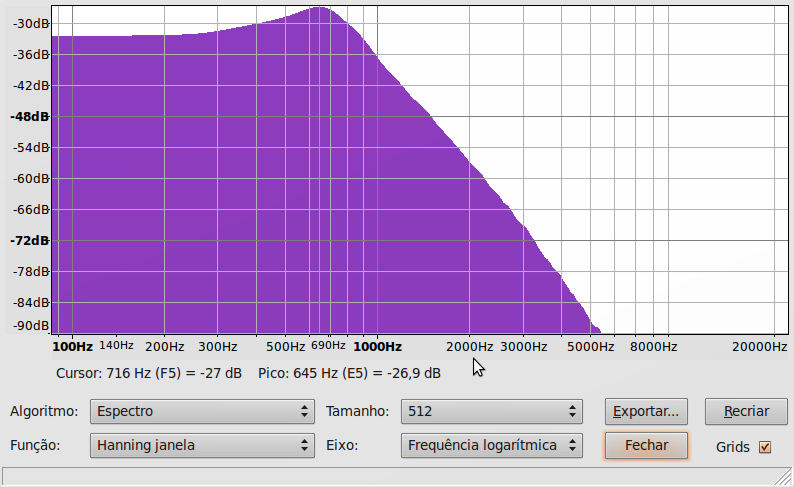
\includegraphics[scale=0.15]{q15.png}
      }%
\qquad
\parbox{1.5in}{
      \centering
      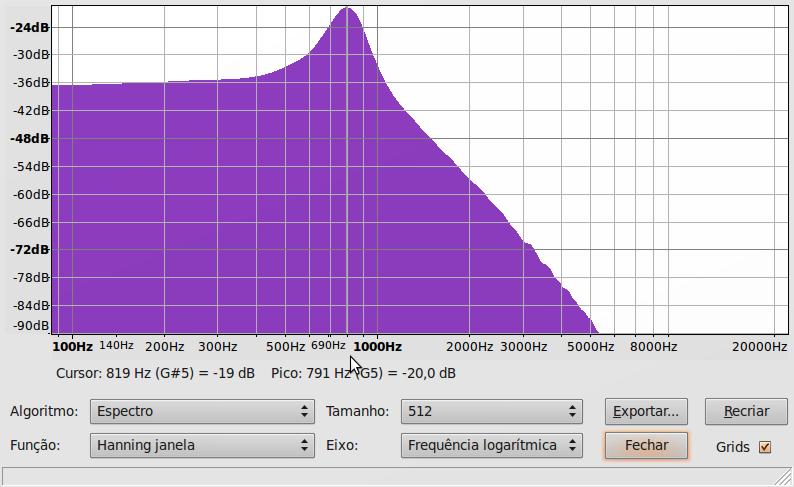
\includegraphics[scale=0.15]{q3.png}
      }%

  \caption{Análise de frequência para q=0.0, 1.5 e 3.0}
  \label{fig:qs}
\end{figure}



De acordo com a figura \ref{fig:qs}, pode-se verificar que a medida que o fator de qualidade aumenta, o espectro de frequência na tem um
 máximo cada vez mais acentuado por volta da frequência de corte, tornando o filtro de um passa baixa para um passa baixa com acentuação na 
banda da frequência de corte.



\begin{figure}
  \centering
\parbox{2in}{
    \centering
    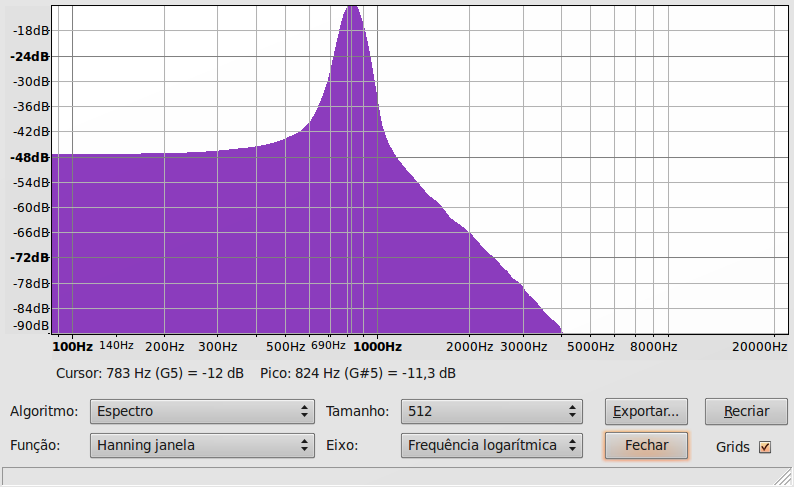
\includegraphics[scale=0.2]{q356.png}
    }%
\qquad	  
\parbox{2in}{
      \centering
      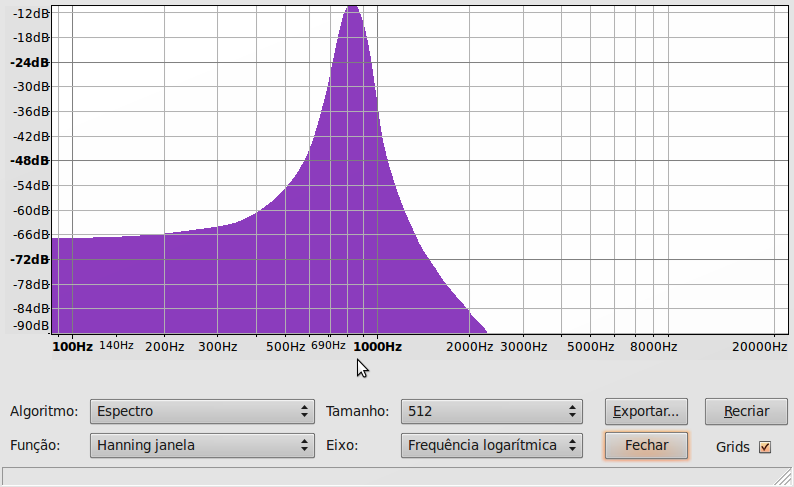
\includegraphics[scale=0.2]{q357.png}
      }%

  \caption{Análise de frequência para q=3.56 e para 3.57}
  \label{fig:qs2}
\end{figure}


A figura \ref{fig:qs2} mostra a situação onde o filtro começa a oscilar sozinho. Para o fator de qualidade igual a $3.56$, a resposta de frequência
do filtro tem a forma igual ao que se tinha, só que com a acentuação na frequência de corte. Com o fotaro de qualidade igual a $3.57$ o comportamento 
do espectro de frequência  do filtro ja é bem diferente. A acentuação em torno da frequência de corte se torna muito maior. 


Os resultados em arquivos de
áudio sempre deram clip após certo tempo com valores de fator de qualidade acima desse patamar, mesmo quando se desliga o sinal de entrada do filtro.
 O filtro perde a característica \emph{FIR}, resposta finita ao impulso, e adquire a característica de um \emph{IIR}, com resposta infinita ao impulso.



\section{A classe \emph{Moog}}
A classe \emph{Moog}, implementada nos arquivos \emph{Moog.cpp} e \emph{Moog.h}, é uma classe que monta toda a arquitetura do minimoog usando os blocos que foram definidos.

\subsection{Os blocos utilizados}
Um construtor da classe Moog cria 2 osciladores, \emph{oscil1} e \emph{oscil2}, com números para controlar frequência e amplitude, um gerador de ruído \emph{noise} 
e um número pra controlar a amplitude, um filtro \emph{filter} e números pra controlar o contorno do filtro, frequência e o fator de qualidade, 2 ADSR, um para controle da 
envoltória de amplitude \emph{env} e outro pra controle da envoltória de frequência \emph{env\_freq}, 2 somadores \emph{adder} e \emph{adder\_aux}, 2 multiplicadores
\emph{mult\_aux} e \emph{mult\_aux2} e um número \emph{master\_amp} pra controlar a amplitude geral.

\subsection{Conexão dos blocos}
Com todos esses blocos criados, a classe Moog conecta a fim de formar a arquitetura do minimoog. Ao criar um objeto da classe Moog, ele inicializa 
cada um dos blocos com valores padão e conecta os blocos.



Para os osciladores e o gerador de ruído, o construtor da classe Moog seleciona os números que controlam a frequência e amplitude como as entradas dos
2 osciladores \emph{oscil1} e \emph{oscil2}, e seleciona \emph{oscil2} como escravo de \emph{oscil1}. Seleciona o número que controla a amplitude do gerador de 
ruído \emph{noise}. Seleciona \emph{oscil1}, \emph{oscil2} e \emph{noise} como as 3 entradas do somador \emph{adder}. 



Para o filtro, a classe Moog usa o multiplicador \emph{mult\_aux} para multiplicar o número que controla o contorno do filtro, com a envoltória de 
frequência \emph{env\_freq} e a frequência de corte, a saída desse multiplicador é somada a frequência de corte com o somador \emph{adder\_aux}.
Para o filtro \emph{filter} é selecionado como sinal de entrada a saída do somador dos osciladores e ruído \emph{adder}, selecionado como frequência 
de corte o segundo somador \emph{adder\_aux} e como fator de qualidade, o número que controla o fator de qualidade. Por último, é usado o multiplicador 
\emph{mult\_aux2} para multiplicar a saída de \emph{filter} com o ADSR \emph{env} e com o controlador de amplitude geral \emph{master\_amp}. 

  
\subsection{Métodos}
A classe Moog também tem métodos para que se possa controlar o valor desses blocos e fazer o controle dos parâmetros do minimoog, que são
 para os osciladores a frequência, amplitude, tipo de forma de onda, a oitava, setar ligado ou desligado, isso para ambos osciladores.
Para o gerador de ruído, os parâmetros são a amplitude, setar ligado ou desligado e o tipo de ruído (branco ou rosa).


Para o filtro o controle é na frequência de corte, o contorno do filtro, o fator de qualidade, setar ligado ou desligado, além do controle
 de ataque, decaimento, sustentação e relaxamento da envoltória de frequência do filtro.
Há ainda o controle para a envoltória de amplitude usada na saída do filtro, que controla o tempo de ataque, decaimento, sustentação e 
relaxamento e o nível de sustentação da envoltória de amplitude.


Então com o uso dos métodos da classe Moog é possivel controlar todos os parâmetros do minimoog.



A classe Moog é apenas uma forma de conectar e controlar os blocos básicos de acordo com a arquitetura do Minimoog, 
então se torna possível formar qualquer tipo de arquitetura 
 de áudio que use os mesmos blocos básicos definidos.





\section{VST}
Nesta seção, temos como objetivo 
descrever como foi feito interfaceamento entre o arcabouço que foi montado 
para a síntese de áudio e a API VST.



Com objetivo de facilitar as questões de compilação e geração de \emph{dll}s 
utilizou-se o Visual Studio para gerenciar o projeto. Instruções para configurar 
o Visual Studio para trabalhar com \emph{plugins} VSTs podem ser encontradas em 
\url{http://www.teragon.org/2010/02/how-to-make-vst-plugins-in-visual.html}.

Nesta parte do sistema, há apenas dois arquivos: \emph{MoogPlugin.h} e \emph{MoogPlugin.cpp}.
No arquivo \emph{MoogPlugin.h} está a declaração da classe \emph{MoogPlugin} que 
extende a classe \emph{AudioEffectX}, que é fornecida pelo SDK. Esta classe instancia 
um objeto da classe \emph{Moog} e gerencia-o. Além disso, é 
definido o número parâmetros que o plugin possui por meio da macro \emph{NUM\_PARAMS}.

A implementação da classe MoogPlugin é feita no arquivo \emph{MoogPlugin.cpp}. Alguns 
métodos importantes:

\begin{itemize}
	\item \emph{processReplacing} - Este é o único método que é obrigatório a implementação 
	por todas as classes que herdam da classe \emph{AudioEffectX}. Este método recebe como parâmetro 
	um buffer de entrada, um buffer de saída, o número de amostras. No buffer de saída são colocadas 
	as amostras geradas pela classe \emph{Moog}
	\item \emph{processEvents} - Este é o método responsável por tratar os eventos VST. 
	Os eventos MIDI são encapsulados dentro de um evento VST, então, é justamente nesse 
	método que as mensagens MIDI são tratadas. Em particular, as mensagens de NoteON e 
	NoteOFF.
	\item \emph{setParameter,getParameter,getParameterLabel,getParameterDisplay,getParameterName} - 
	Estes são os métodos que o \emph{host} do VST chama para configurar os parâmetros do plugin. 
	Todos esses métodos recebem como primeiro argumento um VstInt32 (\emph{index}) que indica qual 
	parâmetros será modificado ou lido. Por exemplo, para modificar o primeiro parâmetro 
	do plugin, o host chamará um desses métodos com \emph{index}$=0$.
\end{itemize}

Todo plugin VST deve prover uma implementação da função \emph{createEffectInstance} e isso 
é feito também no arquivo \emph{MoogPlugin.cpp}. No caso deste projeto, a única coisa 
que é feita nesse método é criar uma objeto da classe \emph{MoogPlugin}. 


\bibliographystyle{IEEEtran}
\bibliography{bibliografia}
\end{document}

